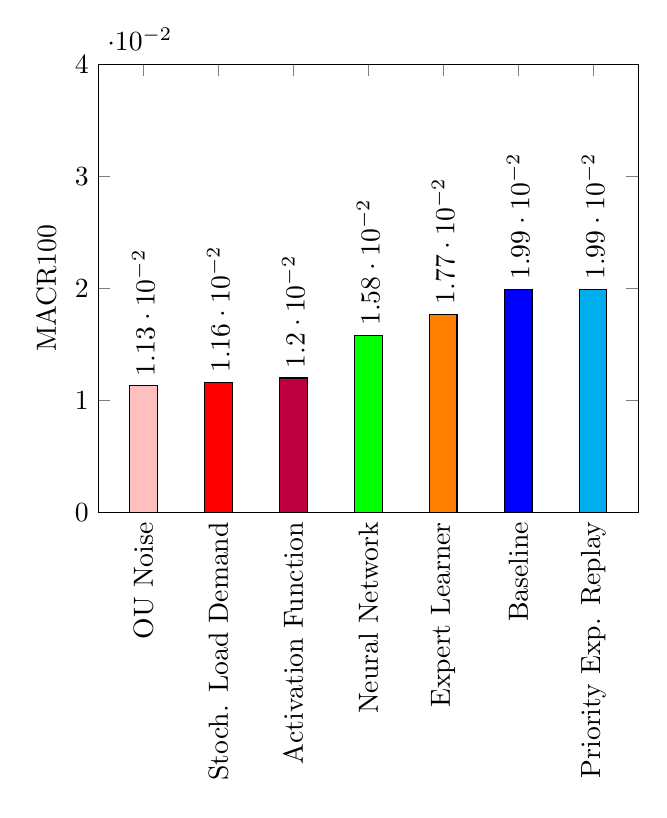
\begin{tikzpicture}
	\begin{axis}[
	    ylabel={MACR100},
	    symbolic x coords={OU Noise,, Stoch. Load Demand,, Activation Function,, Neural Network,, Expert Learner,, Baseline,, Priority Exp. Replay},
	    xtick = {Baseline, Neural Network, Activation Function, OU Noise, Priority Exp. Replay, Expert Learner, Stoch. Load Demand},
	    xticklabel style={rotate=90},
	    nodes near coords,
	    nodes near coords align={vertical},
	    every node near coord/.append style={rotate=90, anchor=west},
	    ymin=0, ymax=0.04
	    ]
	\addplot [ybar, fill=blue] coordinates {(Baseline, 0.0199)};
	\addplot [ybar, fill=green] coordinates {(Neural Network, 0.0158)};
	\addplot [ybar, fill=purple] coordinates {(Activation Function, 0.012)};
	\addplot [ybar, fill=pink] coordinates {(OU Noise, 0.0113)};
	\addplot [ybar, fill=cyan] coordinates {(Priority Exp. Replay, 0.0199)};
	\addplot [ybar, fill=orange] coordinates {(Expert Learner, 0.0177)};
	\addplot [ybar, fill=red] coordinates {(Stoch. Load Demand, 0.0116)};
	%\legend{Baseline, Neural Network, Activation Function, OU Noise, Priority Experience Replay, Expert Learner, Stochastic Load Demand};
	\end{axis}
\end{tikzpicture}